%%%%%%%%%%%%%%%%%%%%%%
%
%   Work related to the verification of the datasets
%
%%%%%%%%%%%%%%%%%%%%%%

\section{Slices of Datacubes}

  \begin{figure}
    \centering
    \includeimage[width=\linewidth]{cube_slices_seed}
    \caption{Slice 0}
  \end{figure}

\section{Powerspectra from Simulations}

  \begin{figure}
      \centering
      % 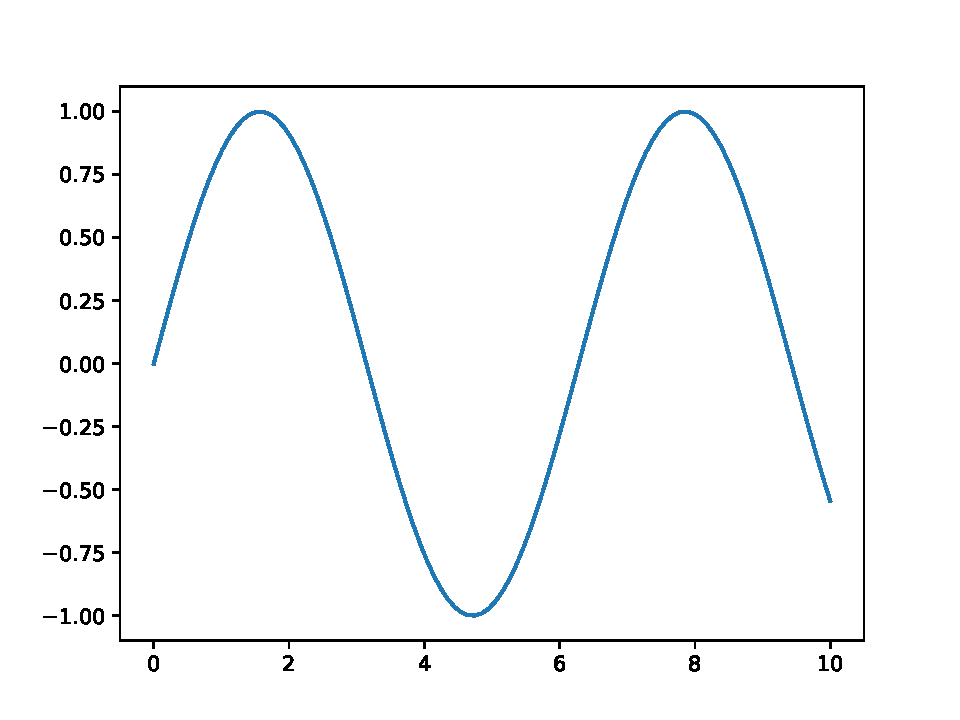
\includegraphics[width=\linewidth]{main/test.pdf}
      \includeimage[width=\linewidth]{average_matter_power_spectra}
      \caption{Average matter power spectra at different redshifts.}
    \end{figure}

    \begin{figure}
      \centering
      % 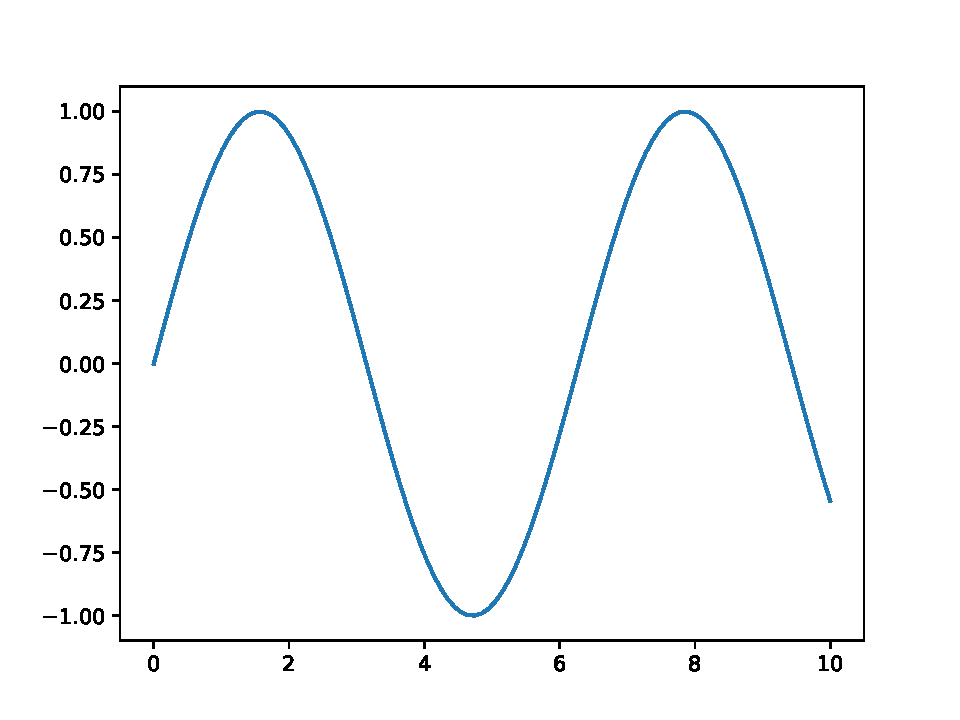
\includegraphics[width=\linewidth]{main/test.pdf}
      \includeimage[width=\linewidth]{average_potential_power_spectra}
      \caption{Average potential power spectra at different redshifts.}
    \end{figure}

\section{Powerspectra from Datacubes}

\section{Analytical Bispectra}

  


  \begin{figure}
    \centering
    \includeimage[width=\linewidth]{analytical_bispectra}
  \end{figure}

\section{Bispectra from Cube}
  \subsection{Binning}
    % \begin{equation}
    %   k_\mathrm{new
    % \end{equation}

    \begin{figure}
      \centering
      \includeimage[width=\linewidth]{binning_example}
    \end{figure}

  \subsection{Bispectra}
    \begin{figure}
      \centering
      \includeimage[width=\linewidth]{average_bispectra}
    \end{figure}


